%%%%%%%%%%%%%%%%%%%%%%%%%%%%%%%%%%%%%%%%%%%%%%%%%%%%%%%%%%%%%%%%%%%%%%%%%%%%%%%%
%%%%%%%%%%%%%%%%%%%%%%%%%%%%%%%%%%%%%%%%%%%%%%%%%%%%%%%%%%%%%%%%%%%%%%%%%%%%%%%%
\clearpage
\section{Design development - control design}\label{sec:controller}
\tikzset{%
  block/.style    = {draw, thick, rectangle, minimum height = 3em,
    minimum width = 3em},
  sum/.style      = {draw, circle, node distance = 2cm}, % Adder
  input/.style    = {coordinate}, % Input
  output/.style   = {coordinate} % Output
}
%%%%%%%%%%%%%%%%%%%%%%%%%%%%%%%%%%%%%%%%%%%%%%%%%%%%%%%%%%%%%%%%%%%%%%%%%%%%%%%%
\paragraph{Introduction}
~\\
Our system description works on the basis of a model perturbed from steady-state. The operating point that the model is linearised about is defined by a steady-state duty ratio $D$, steady-state input vector $U$ (which contains the steady-state values for the converter circuit input voltage $v_g$ and diode voltage $V_D$), and the component values $L_1$, $L_2$, $C_1$, $C_2$, $R_1$, $R_2$, $R_3$, $R_4$, $R_o$, $R_D$, and $R$.
\newpar
The steady-state values defining the operating point as used in the controller as implemented in the product are provided in Sections~\ref{sec:system_params} and~\ref{sec:control_params}, while the reasoning behind and effects of the values they take are discussed in Section~\hl{[TODO find section discussing selection of operating point]}.
\newpar
These quantities determines matrices $\boldsymbol{A}$, $\boldsymbol{b}$, $\boldsymbol{b}_d$, $\boldsymbol{c}$, the steady-state input vector $\boldsymbol{U}$, the steady-state state vector $\boldsymbol{X}$, and the steady-state output $\boldsymbol{Y}$.
\newpar
This section will outline the approach taken in designing a continuous-time controller utilising observer state feedback and integral action. The resulting controller will be discretised under a regime appropriate for implementation on a microcontroller.
\paragraph{Notation}
\begin{itemize}
    \item
        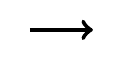
\begin{tikzpicture}[scale = 0.8]
        \draw[->, ultra thick] (0,0) -- (1,0);
        \end{tikzpicture}
        (thick line): vector quantity
\end{itemize}
%%%%%%%%%%%%%%%%%%%%%%%%%%%%%%%%%%%%%%%%%%%%%%%%%%%%%%%%%%%%%%%%%%%%%%%%%%%%%%%%
\subsection{Open-loop: a model to estimate time-varying perturbations}
Every state variable in the state-space averaged model of a DC-DC converter circuit is the sum of a steady-state and time-varying component. The steady-state components are calculated according to Equation~(\ref{eqn:modelY}), while our model estimates the values of the time-varying components.
\begin{figure}[H]
\centering
\fbox{
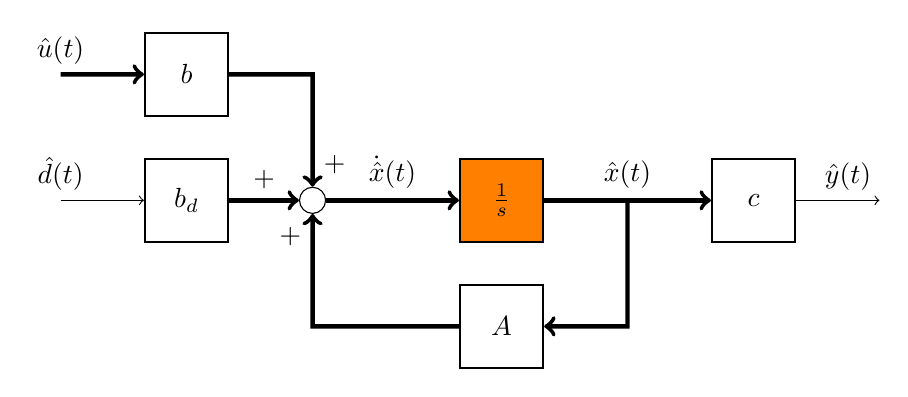
\begin{tikzpicture}[scale = 0.8]
%blocks
\draw
	(2,2) node [block] (bb) {$\boldsymbol{b}$}
	(4,0) node [sum] (s1) {\suma}
	(7,0) node [block, fill = orange] (i1) {$\frac{1}{s}$}
	(7,-2) node [block] (bA) {$\boldsymbol{A}$}
	(2,0) node [block] (bbD) {$\boldsymbol{b}_d$}
	(11,0) node [block] (bc) {$\boldsymbol{c}$};
%lines
\draw[->, ultra thick] (0,2) -- (bb);
\draw[->, ultra thick] (bb) -- (4,2) -- node [anchor = west, pos = 0.8] {$+$} (s1);
\draw[->, ultra thick] (s1) -- node [above] {$\dot{\hat{\boldsymbol{x}}}(t)$} (i1);
\draw[->, ultra thick] (i1) -- node [above] {$\hat{\boldsymbol{x}}(t)$} (bc);
\draw[->, ultra thick] (9,0) -- (9,-2) -- (bA);
\draw[->, ultra thick] (bA) -- (4,-2) -- node [anchor = east, pos = 0.8] {$+$} (s1);
\draw[->] (bc) -- (13,0);
%more lines
\draw[->] (0,0) -- (bbD);
\draw[->, ultra thick] (bbD) -- node [anchor = south, pos = 0.5] {$+$} (s1);
%labels
\coordinate[label = above:$\hat{\boldsymbol{u}}(t)$] (u) at (0,2);
\coordinate[label = above:$\hat{d}(t)$] (hatd) at (0,0);
\coordinate[label = above:$\hat{y}(t)$] (haty) at (12.5,0);
\end{tikzpicture}
}
\caption{Block diagram representation of Equation~(\ref{eqn:timevarying2})}
\label{block:openloop}
\end{figure}
The block diagram of Figure~\ref{block:openloop} is a representation of the relationship between the time-varying components of the state variables.
\newpar
It is desired to achieve control of the model in Figure~\ref{block:openloop}. A reasonable control regime to be investigated first is that of full-state feedback. Full-state feedback operates by generating a (scalar) control signal as the product of a (horizontal) gain matrix $\boldsymbol{K}$ and the (vertical) state vector $\boldsymbol{x}$ (where $\boldsymbol{K}$ contains the same number of entries as $\boldsymbol{x}$). In controlling a DC-DC converter circuit, this control signal will be the duty ratio $d$, and in the model of the \'Cuk converter, this duty ratio (or rather the time-varying component of it) will enter the system by the matrix $\boldsymbol{b}_d$. The entries of the gain matrix $\boldsymbol{K}$ are determined according to desired closed-loop transient performance, and there exists many methods for computing them (e.g pole-placement, LQR, loop shaping).
\newpar
Therefore, values of the states comprising the state vector (i.e. $v_{C1}$, $v_{C2}$, $i_{L1}$, and $i_{L2}$ in the \'Cuk converter) at every point in time\footnote{Note that in discrete time (see Section~\ref{sec:disc}) the equivalent is that values of the states are required at the transition between every successive integer time-step.}, are required to implement full-state feedback. The most straightforward method of obtaining this information is to implement sensors in hardware to measure $v_{C1}$, $v_{C2}$, $i_{L1}$, and $i_{L2}$.
\newpar
Sensors for measuring capacitor voltages would be relatively simple to implement. Indeed, our product uses voltage sensing circuitry to measure the converter circuit input and output voltages $v_g$ and $v_o$\footnote{See Section~\ref{sec:voltagesensing}.}. However, the states $v_{C1}$ and $v_{C2}$ are defined as the voltages across the ideal capacitor elements $C_1$ and $C_2$ (that is, as decoupled from their respective ESR elements). It is not possible to build a sensor in hardware that would measure these ideal voltages\footnote{Although they could theoretically be estimated through knowledge of the capacitor parasitic resistances $R_3$ and $R_4$.}. Additionally, current sensors for the inductors would require the introduction of current sense resistors\footnote{Measuring current through the measuring of the voltage drop across a current sense resistor is the hardware sensor implementation most relevant in the measuring of $i_{L1}$ and $i_{L2}$.} in series with the inductors $L_1$ and $L_2$. As will be discussed in Section~\hl{[TODO find section on why low parasitic important]}, this degrades the conversion ratio from input to output voltages in the converter circuit.
\newpar
Thus a Luenberger observer will be investigated as a method for obtaining estimates of the state vector to permit the implementation of full-state (now observer) feedback.
%%%%%%%%%%%%%%%%%%%%%%%%%%%%%%%%%%%%%%%%%%%%%%%%%%%%%%%%%%%%%%%%%%%%%%%%%%%%%%%%
%%%%%%%%%%%%%%%%%%%%%%%%%%%%%%%%%%%%%%%%%%%%%%%%%%%%%%%%%%%%%%%%%%%%%%%%%%%%%%%%
\subsection{Estimating voltages and currents for full-state feedback: the Luenberger observer}
% A Luenberger observer may be used to produce estimates of the time-varying components of the system states which may then be employed in a full-state feedback closed-loop control regime.
% \newpar
A system is said to be observable (i.e. has no unobservable states) if the observability matrix as defined in Equation~(\ref{eqn:observable}) has full rank. For a $n$-state SISO system this may easily be checked using the \textsf{MATLAB} call of~(\ref{matlab:observable})\footnote{It was decided not to include the detailed workings of observability in this report in favour of including greater discussion on hardware, programming, and implementation.}.
\begin{align}
\mathcal{O}
=
\begin{bmatrix}
\boldsymbol{c} \\
\boldsymbol{c}\boldsymbol{A} \\
\boldsymbol{c}\boldsymbol{A}^2 \\
\vdots \\
\boldsymbol{c}\boldsymbol{A}^{n - 1}
\end{bmatrix}
\qquad
\text{for a system with } n \text{ states}
\label{eqn:observable}
\end{align}
%
\begin{align}
\texttt{rank(obsv(A, c)) == n}
\label{matlab:observable}
\end{align}
\rule{\textwidth}{0.5pt}
\begin{align}
\boldsymbol{\dot{\hat{x}}}_\ell (t) &= \boldsymbol{A}\hat{\boldsymbol{x}}_\ell(t) + \boldsymbol{b}\hat{\boldsymbol{u}}(t) + \boldsymbol{b}_d \hat{d}(t) + \boldsymbol{L}\squarey{\hat{y}(t) - \hat{y}_\ell(t)},
\label{eqn:observer}
\\[11pt]
\boldsymbol{\dot{\hat{x}}}_\ell (t) &= \squarey{\boldsymbol{A} - \boldsymbol{L}\boldsymbol{c}}\hat{\boldsymbol{x}}_\ell(t) + \boldsymbol{b}\hat{\boldsymbol{u}}(t) + \boldsymbol{b}_d \hat{d}(t) + \boldsymbol{L}\hat{y}(t).
\label{eqn:observer2}
\end{align}
For an observable system modelled through the technique of state-space averaging, an estimate of the perturbed state vector may be obtained by extracting the state vector in the system described according to Equation~(\ref{eqn:observer}) and the equivalent Equation~(\ref{eqn:observer2}), where
\begin{itemize}
    \item $\boldsymbol{x}_\ell(t)$: vector containing state estimates
    \item $y(t)$: output state
    \begin{itemize}
        \item for a DC-DC converter circuit this value is obtained through measurement in hardware
    \end{itemize}
    \item $\hat{y}(t) = y(t) - Y$ where $Y$ is the steady-state component of the output state as predicted by the converter circuit model according to Equation~(\ref{eqn:modelY})
    \item $\hat{\boldsymbol{u}}(t) = \boldsymbol{u}(t) - \boldsymbol{U}$
    \begin{itemize}
        \item for the \'Cuk converter modelled with the diode forward voltage drop, $\boldsymbol{u}(t) - \boldsymbol{U} = \begin{bmatrix}v_g - V_g & 0 & 0 & 0\end{bmatrix}$ where $v_g$ is the converter circuit input voltage as measured in hardware and $V_g$ is the converter circuit input voltage as used in defining the operating point to linearise the model about
    \end{itemize}
    \item $\boldsymbol{L}$: observer gain matrix
\end{itemize}
If $\squarey{\boldsymbol{A} - \boldsymbol{L}\boldsymbol{c}}$ is stable, then the error between the estimated and actual system states decays to 0 exponentially. Under this condition the estimated system states may replace the actual system states in a full-state feedback regime.
\newpar
The observer gain matrix is typically populated such that the eigenvalues of $\boldsymbol{A} - \boldsymbol{L}\boldsymbol{c}$ are at least $10 \times$ faster than the eigenvalues of the closed-loop feedback system. This may be done using pole placement, where the poles are chosen to achieve this speed of the observer dynamics. A call to \textsf{MATLAB}'s \texttt{acker} function as
\begin{align}
\texttt{L = acker(A', c', [p p \ldots p])'} \qquad \text{(n-}\texttt{p}\text{'s)},
\label{matlab:place}
\end{align}
where \texttt{p} denotes pole location, is a simple method for populating the observer gain matrix for a $n$-state system. Note that $(\quad\texttt{'}\quad)$ denotes transposition.
%%%%%%%%%%%%%%%%%%%%%%%%%%%%%%%%%%%%%%%%%%%%%%%%%%%%%%%%%%%%%%%%%%%%%%%%%%%%%%%%
The block diagram representation of Equation~(\ref{eqn:observer}) is given in Figure~\ref{block:observer}.
\begin{figure}[H]
\centering
\fbox{
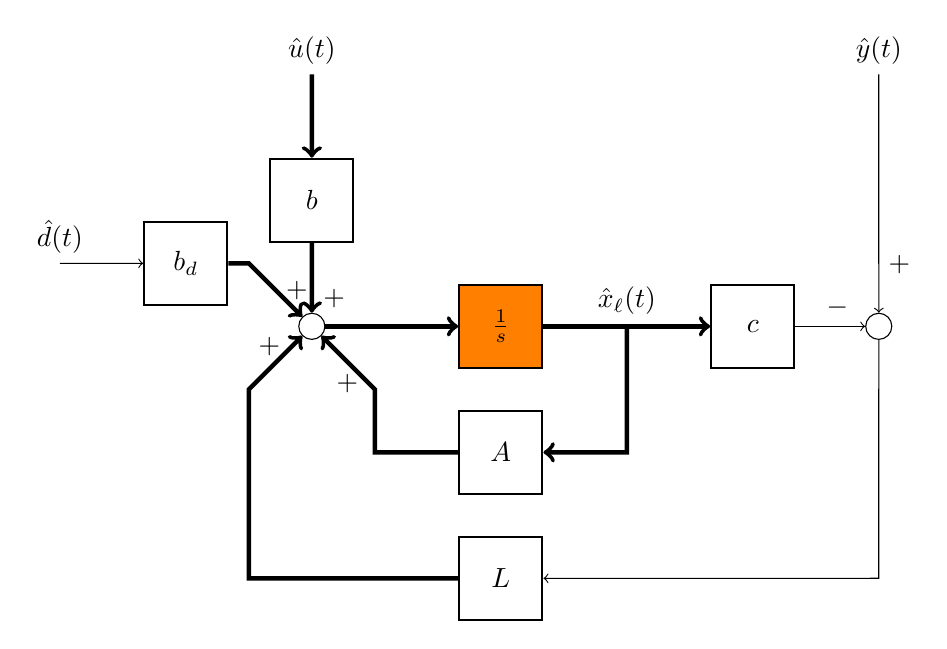
\begin{tikzpicture}[scale = 0.8]
%observer blocks
\draw
	(4,2) node [block] (bb) {$\boldsymbol{b}$}
	(4,0) node [sum] (s1) {\suma}
	(7,0) node [block, fill = orange] (i1) {$\frac{1}{s}$}
	(7,-2) node [block] (bA) {$\boldsymbol{A}$}
	(7,-4) node [block] (bL) {$\boldsymbol{L}$}
	(2,1) node [block] (bbD) {$\boldsymbol{b}_d$}
	(11,0) node [block] (bc) {$\boldsymbol{c}$};
%observer lines
\draw[->, ultra thick] (4,4) -- (bb);
\draw[->, ultra thick] (bb) -- node [anchor = west, pos = 0.8] {$+$} (s1);
\draw[->, ultra thick] (s1) -- (i1);
\draw[->, ultra thick] (i1) -- node [above] {$\hat{\boldsymbol{x}}_\ell(t)$} (bc);
\draw[->, ultra thick] (9,0) -- (9,-2) -- (bA);
\draw[->, ultra thick] (bA) -- (5,-2) -- (5,-1) -- node [anchor = east, pos = 0.1] {$+$} (s1);
\draw[->, ultra thick] (bbD) -- (3,1) -- node [anchor = south, pos = 0.9] {$+$} (s1);
%more observer blocks
\draw (13,0) node [sum] (sobserve) {\suma};
%more observer lines
\draw[->] (sobserve) -- (13,-4) -- (bL);
\draw[->, ultra thick] (bL) -- (3,-4) -- (3,-1) -- node [anchor = east, pos = 0.8] {$+$} (s1);
\draw[->] (bc) -- node [anchor = south, pos = 0.6] {$-$} (sobserve);
\draw[->] (13,4) -- node [anchor = west, pos = 0.8] {$+$} (sobserve);
\draw[->] (0,1) -- (bbD);
%signal labels
\coordinate[label = above:$\hat{d}(t)$] (d) at (0,1);
\coordinate[label = above:$\hat{\boldsymbol{u}}(t)$] (u) at (4,4);
\coordinate[label = above:$\hat{y}(t)$] (yhat) at (13,4);
\end{tikzpicture}
}
\caption{Block diagram representation of Equation~\ref{eqn:observer}}
\label{block:observer}
\end{figure}
%%%%%%%%%%%%%%%%%%%%%%%%%%%%%%%%%%%%%%%%%%%%%%%%%%%%%%%%%%%%%%%%%%%%%%%%%%%%%%%%
\begin{figure}[H]
\centering
\fbox{
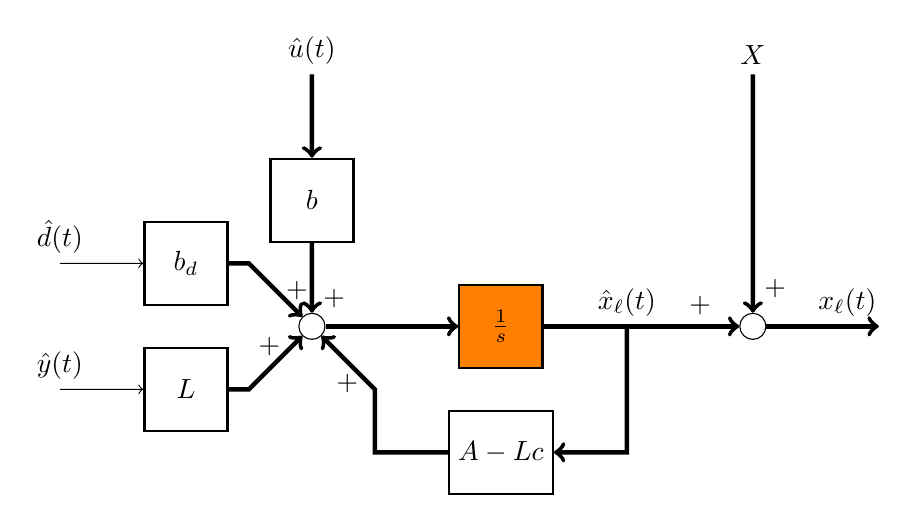
\begin{tikzpicture}[scale = 0.8]
%observer blocks
\draw
	(4,2) node [block] (bb) {$\boldsymbol{b}$}
	(4,0) node [sum] (s1) {\suma}
	(7,0) node [block, fill = orange] (i1) {$\frac{1}{s}$}
	(7,-2) node [block] (bA) {$\boldsymbol{A} - \boldsymbol{L}\boldsymbol{c}$}
	(2,-1) node [block] (bL) {$\boldsymbol{L}$}
	(2,1) node [block] (bbD) {$\boldsymbol{b}_d$}
	(11,0) node [sum] (s2) {\suma};
%observer lines
\draw[->, ultra thick] (4,4) -- (bb);
\draw[->, ultra thick] (bb) -- node [anchor = west, pos = 0.8] {$+$} (s1);
\draw[->, ultra thick] (s1) -- (i1);
\draw[->, ultra thick] (i1) -- node [anchor = south, pos = 0.8] {$+$} (s2);
\draw[->, ultra thick] (9,0) -- (9,-2) -- (bA);
\draw[->, ultra thick] (bA) -- (5,-2) -- (5,-1) -- node [anchor = east, pos = 0.1] {$+$} (s1);
\draw[->, ultra thick] (bbD) -- (3,1) -- node [anchor = south, pos = 0.9] {$+$} (s1);
%more observer lines
\draw[->, ultra thick] (bL) -- (3,-1) -- node [anchor = east, pos = 0.8] {$+$} (s1);
\draw[->] (0,1) -- (bbD);
\draw[->] (0,-1) -- (bL);
\draw[->, ultra thick] (11,4) -- node [anchor = west, pos = 0.9] {$+$} (s2);
\draw[->, ultra thick] (s2) -- (13,0);
%signal labels
\coordinate[label = above:$\hat{d}(t)$] (d) at (0,1);
\coordinate[label = above:$\hat{\boldsymbol{u}}(t)$] (u) at (4,4);
\coordinate[label = above:$\hat{y}(t)$] (yhat) at (0,-1);
\coordinate[label = above:$\boldsymbol{X}$] (bigx) at (11,4);
\coordinate[label = above:$\boldsymbol{x}_\ell(t)$] (smallx) at (12.5,0);
\coordinate[label = above:$\hat{\boldsymbol{x}}_\ell(t)$] (hatx) at (9,0);
\end{tikzpicture}
}
\caption{Block diagram representation of Equation~\ref{eqn:observer2}}
\label{block:observer2}
\end{figure}
The system of Figure~\ref{block:observer} may be represented in a slightly different way that is of more relevance under discretisation. This different representation is provided in Figure~\ref{block:observer2}. Blocks to extract the true state estimate (i.e. sum of transient and steady-state) are introduced also. This system is described by Equation~(\ref{eqn:observer2}). The state vector $\boldsymbol{x}_l (t)$ contains the estimates of the internal system states, while $\hat{\boldsymbol{x}}_l (t)$ may be fed back under full-state feedback to achieve desirable closed-loop performance.
%%%%%%%%%%%%%%%%%%%%%%%%%%%%%%%%%%%%%%%%%%%%%%%%%%%%%%%%%%%%%%%%%%%%%%%%%%%%%%%%
%%%%%%%%%%%%%%%%%%%%%%%%%%%%%%%%%%%%%%%%%%%%%%%%%%%%%%%%%%%%%%%%%%%%%%%%%%%%%%%%
\subsection{Closing the loop: observer state feedback}
With the observer system now described in general terms\footnote{Population of the observer gain matrix $\boldsymbol{L}$ will occur in Section~\ref{sec:simulation_specifications}.}, state feedback control may be investigated.
\begin{figure}[H]
\centering
\fbox{
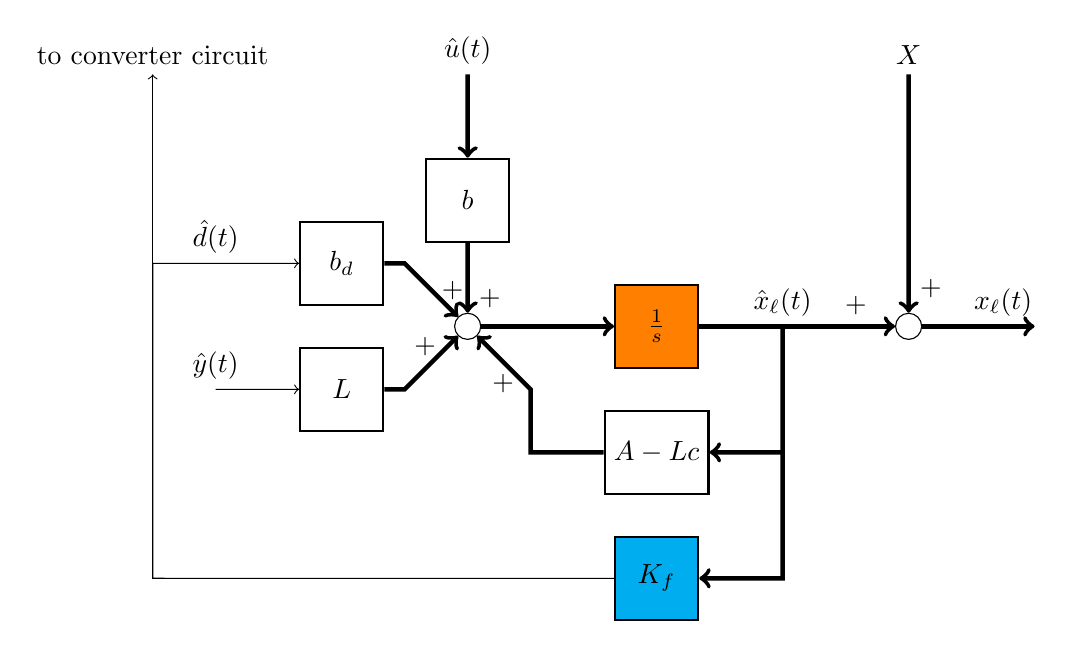
\begin{tikzpicture}[scale = 0.8]
% blocks
\draw
	(4,2) node [block] (bb) {$\boldsymbol{b}$}
	(4,0) node [sum] (s1) {\suma}
	(7,0) node [block, fill = orange] (i1) {$\frac{1}{s}$}
	(7,-2) node [block] (bA) {$\boldsymbol{A} - \boldsymbol{L}\boldsymbol{c}$}
	(2,-1) node [block] (bL) {$\boldsymbol{L}$}
	(2,1) node [block] (bbD) {$\boldsymbol{b}_d$}
	(11,0) node [sum] (s2) {\suma}
	(7,-4) node [block, fill = cyan] (bKf) {$\minus \boldsymbol{K}_f$};
% observer lines
\draw[->, ultra thick] (4,4) -- (bb);
\draw[->, ultra thick] (bb) -- node [anchor = west, pos = 0.8] {$+$} (s1);
\draw[->, ultra thick] (s1) -- (i1);
\draw[->, ultra thick] (i1) -- node [anchor = south, pos = 0.8] {$+$} (s2);
\draw[->, ultra thick] (9,0) -- (9,-2) -- (bA);
\draw[->, ultra thick] (bA) -- (5,-2) -- (5,-1) -- node [anchor = east, pos = 0.1] {$+$} (s1);
\draw[->, ultra thick] (bbD) -- (3,1) -- node [anchor = south, pos = 0.9] {$+$} (s1);
% more observer lines
\draw[->, ultra thick] (bL) -- (3,-1) -- node [anchor = east, pos = 0.8] {$+$} (s1);
\draw[->] (0,-1) -- (bL);
\draw[->, ultra thick] (11,4) -- node [anchor = west, pos = 0.9] {$+$} (s2);
\draw[->, ultra thick] (s2) -- (13,0);
% signal labels
\coordinate[label = above:$\hat{d}(t)$] (d) at (0,1);
\coordinate[label = above:$\hat{\boldsymbol{u}}(t)$] (u) at (4,4);
\coordinate[label = above:$\hat{y}(t)$] (yhat) at (0,-1);
\coordinate[label = above:$\boldsymbol{X}$] (bigx) at (11,4);
\coordinate[label = above:$\boldsymbol{x}_\ell(t)$] (smallx) at (12.5,0);
\coordinate[label = above:$\hat{\boldsymbol{x}}_\ell(t)$] (hatx) at (9,0);
% feedback lines
\draw[->, ultra thick] (9,-2) -- (9,-4) -- (bKf);
\draw[->] (bKf) -- (-1,-4) -- (-1,1) -- (bbD);
% more lines
\draw[->] (-1,1) -- (-1,4);
% more labels
\coordinate[label = above:{to converter circuit}] (dout) at (-1,4);
\end{tikzpicture}
}
% \caption[Caption without FN]{Block diagram representing a system controlled by observer state feedback\footnotemark}
\caption{Block diagram representing a system controlled by observer state feedback}
\label{block:feedback}
\end{figure}
Note that in Figure~\ref{block:feedback} and future block diagrams with lines indicating `to converter circuit' the actual duty ratio as sent to the PWM module is $d(t) = D + \hat{d}(t)$, according to Equation~(\ref{eqn:dDhatd}).
\newpar
%
% \footnotetext{Note that in this and future block diagrams extracting the perturbation in duty ratio $\hat{d}(t)$ the duty ratio as sent to the PWM module is $d(t) = D + \hat{d}(t)$, according to Equation~(\ref{eqn:dDhatd}).}
%
The gain matrix $\boldsymbol{K}_f$ is populated to produce desirable closed-loop performance. Full-state feedback is primarily used to achieve smooth system response to step changes in reference, but produces non-zero steady state error. Thus full-state feedback addresses 1 of the control objectives of Section~\ref{sec:objectives}. The non-zero steady-state error resulting from this scheme may be eliminated by introducing a reference input and integral action, to achieve the respective control objective of Section~\ref{sec:objectives}. The reference input control signal will be the output voltage desired for the converter to achieve.
\newpar
Updating the model for integral action may be achieved by augmenting the state vector with another state representing the integral of the difference between the reference input and measured output. This augmentation approach will be detailed in the following section.
%%%%%%%%%%%%%%%%%%%%%%%%%%%%%%%%%%%%%%%%%%%%%%%%%%%%%%%%%%%%%%%%%%%%%%%%%%%%%%%%
%%%%%%%%%%%%%%%%%%%%%%%%%%%%%%%%%%%%%%%%%%%%%%%%%%%%%%%%%%%%%%%%%%%%%%%%%%%%%%%%
\subsection{Introducing a reference input and integral action}
\begin{figure}[H]
\centering
\fbox{
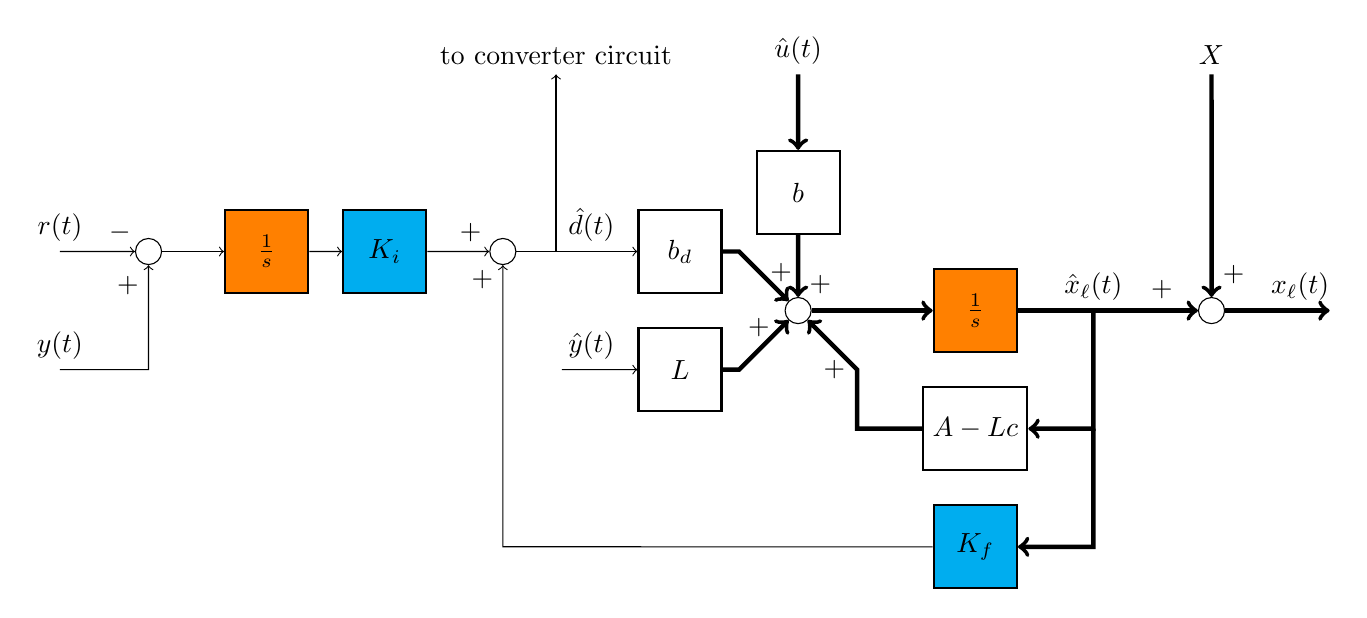
\begin{tikzpicture}[scale = 0.75]
% blocks
\draw
	(4,2) node [block] (bb) {$\boldsymbol{b}$}
	(4,0) node [sum] (s1) {\suma}
	(7,0) node [block, fill = orange] (i1) {$\frac{1}{s}$}
	(7,-2) node [block] (bA) {$\boldsymbol{A} - \boldsymbol{L}\boldsymbol{c}$}
	(2,-1) node [block] (bL) {$\boldsymbol{L}$}
	(2,1) node [block] (bbD) {$\boldsymbol{b}_d$}
	(11,0) node [sum] (s2) {\suma}
	(7,-4) node [block, fill = cyan] (bKf) {$\minus \boldsymbol{K}_f$};
% observer lines
\draw[->, ultra thick] (4,4) -- (bb);
\draw[->, ultra thick] (bb) -- node [anchor = west, pos = 0.8] {$+$} (s1);
\draw[->, ultra thick] (s1) -- (i1);
\draw[->, ultra thick] (i1) -- node [anchor = south, pos = 0.8] {$+$} (s2);
\draw[->, ultra thick] (9,0) -- (9,-2) -- (bA);
\draw[->, ultra thick] (bA) -- (5,-2) -- (5,-1) -- node [anchor = east, pos = 0.01] {$+$} (s1);
\draw[->, ultra thick] (bbD) -- (3,1) -- node [anchor = south, pos = 0.85] {$+$} (s1);
% more observer lines
\draw[->, ultra thick] (bL) -- (3,-1) -- node [anchor = east, pos = 0.85] {$+$} (s1);
\draw[->] (0,-1) -- (bL);
\draw[->, ultra thick] (11,4) -- node [anchor = west, pos = 0.9] {$+$} (s2);
\draw[->, ultra thick] (s2) -- (13,0);
% signal labels
\coordinate[label = above:$\hat{d}(t)$] (d) at (0.5,1);
\coordinate[label = above:$\hat{\boldsymbol{u}}(t)$] (u) at (4,4);
\coordinate[label = above:$\hat{y}(t)$] (yhat) at (0.5,-1);
\coordinate[label = above:$\boldsymbol{X}$] (bigx) at (11,4);
\coordinate[label = above:$\boldsymbol{x}_\ell(t)$] (smallx) at (12.5,0);
\coordinate[label = above:$\hat{\boldsymbol{x}}_\ell(t)$] (hatx) at (9,0);
\coordinate[label = above:$r(t)$] (r) at (-8.5,1);
\coordinate[label = above:$y(t)$] (r) at (-8.5,-1);
% integrator blocks
\draw
    (-1,1) node [sum] (s5) {\suma}
	(-3,1) node [block, fill = cyan] (bKi) {$\minus K_i$}
	(-5,1) node [block, fill = orange] (i2) {$\frac{1}{s}$}
	(-7,1) node [sum] (s4) {\suma};
% feedback lines
\draw[->, ultra thick] (9,-2) -- (9,-4) -- (bKf);
\draw[->] (bKf) -- (-1,-4) -- node [anchor = east, pos = 0.95] {$+$} (s5);
\draw[->] (s5) -- (bbD);
% integrator lines
\draw[->] (-8.5,1) -- node [anchor = south, pos = 0.8] {$-$} (s4);
\draw[->] (s4) -- (i2);
\draw[->] (i2) -- (bKi);
\draw[->] (bKi) -- node [anchor = south, pos = 0.7] {$+$} (s5);
\draw[->] (-8.5,-1) -- (-7,-1) -- node [anchor = east, pos = 0.8] {$+$} (s4);
% more lines
\draw[->] (-0.1,1) -- (-0.1,4);
% more labels
\coordinate[label = above:{to converter circuit}] (dout) at (-0.1,4);
\end{tikzpicture}
}
\caption{Block diagram representing observer state feedback and integral action acting on the model of Equation~(\ref{eqn:timevarying2})}
\label{block:integral}
\end{figure}
% So our microcontroller will estimate the above system and send to the converter a PWM signal of duty ratio $d(t) = \hat{d}(t) + D$ where $D$ is the steady-state duty ratio used in generating a linear model of the system.
%%%%%%%%%%%%%%%%%%%%%%%%%%%%%%%%%%%%%%%%%%%%%%%%%%%%%%%%%%%%%%%%%%%%%%%%%%%%%%%%
% \newpar
Our system description may be updated by augmenting the state vector with an additional state for the integral of the error $\dot{x}_i(t) = e(t) = y(t) - r(t)$ ($x_i(t) = \int \mathrm{d}t \curly{e(t)}$). Then
\begin{align*}
\boldsymbol{\dispdot[0mu]{\hat{x}}_a}(t) &= \boldsymbol{A}_a\hat{\boldsymbol{x}}_a(t) + \boldsymbol{b}_a \hat{\boldsymbol{u}}_a(t) + \boldsymbol{b}_{d_a} \hat{d}(t) + \boldsymbol{r}(t),
\\[11pt]
\hat{y}(t) &= \boldsymbol{c}_a \hat{\boldsymbol{x}}_a(t),
\end{align*}
with
\begingroup
\allowdisplaybreaks
\begin{align}
\hat{\boldsymbol{x}}_a (t) &=
\begin{bmatrix}
\hat{v}_{C1} (t) & \hat{v}_{C2} (t) & \hat{i}_{L1} (t) & \hat{i}_{L2} (t) & x_i (t)
\end{bmatrix}^\intercal,
\\[11pt]
\hat{\boldsymbol{u}}_a (t) &=
\begin{bmatrix}
\hat{\boldsymbol{u}} (t) \\ 0
\end{bmatrix},
\\[11pt]
\boldsymbol{r}(t) &=
\begin{bmatrix}
0 & 0 & 0 & 0 & \minus r(t)
\end{bmatrix}^\intercal,
\\[11pt]
\boldsymbol{A}_a &=
\begin{bmatrix}
\boldsymbol{A} & 0\\
\boldsymbol{c} & 0
\end{bmatrix},
\label{eqn:augmentedA}
\\[11pt]
\boldsymbol{b}_a
&=
\begin{bmatrix}
\boldsymbol{b} \\ 0
\end{bmatrix},
\\[11pt]
\boldsymbol{b}_{d_a}
&=
\begin{bmatrix}
\boldsymbol{b}_d \\ 0
\end{bmatrix},
\label{eqn:augmentedbD}
\\[11pt]
\boldsymbol{c}_a
&=
\begin{bmatrix}
\boldsymbol{c} & 0
\end{bmatrix}.
\end{align}
\endgroup
The control system of Figure~\ref{block:integral} should satisfy the control objectives of Section~\ref{sec:objectives}. What is now required is a method for computing the gains $\boldsymbol{K}_f$ and $K_i$. These gains will determine the poles of the system, and thus the stability and transient behaviour.
%%%%%%%%%%%%%%%%%%%%%%%%%%%%%%%%%%%%%%%%%%%%%%%%%%%%%%%%%%%%%%%%%%%%%%%%%%%%%%%%
%%%%%%%%%%%%%%%%%%%%%%%%%%%%%%%%%%%%%%%%%%%%%%%%%%%%%%%%%%%%%%%%%%%%%%%%%%%%%%%%
\subsection{Linear quadratic regulator (LQR); a method for determining $\boldsymbol{K}_f$ and $K_i$}\label{sec:LQR}
The linear quadratic regulator is a feedback controller that produces the control input to a state-space system according to the following proposition:
~\\~\\
\hspace*{\fill}
\begin{minipage}[t]{0.8\textwidth}
\textit{
Assume that we aim to drive the initial state $x_0$ to the smallest possible value as soon as possible in the interval $[t_0, \, t_f]$, but without spending too much control effort (as measured by the magnitude of $u$) to achieve that goal. Then, the optimal regulator problem is defined as the problem of finding an optimal control $u(t)$ over
the interval $[t_0, \, t_f]$ such that the following cost function is minimized.
}\\
(\cite{controlsystemdesign}, page 663).
\end{minipage}
\hspace*{\fill}
~\\~\\~\\
where the cost function the proposition is referring to is:
\begin{align}
J_u \paren{\boldsymbol{x}(t_0), t_0} = \int_{t_0}^{t_f} \mathrm{d}t\curly{\boldsymbol{x}(t)^\intercal \boldsymbol{Q} \cdot \boldsymbol{x}(t)
+ u(t)^\intercal R \cdot u(t)
+ 2 \boldsymbol{x}(t)^\intercal \boldsymbol{N} \cdot u(t)}.
\label{eqn:LQR}
\end{align}
%
Here (Equation~(\ref{eqn:LQR})) $\boldsymbol{x}(t)$ refers to the system state vector and $u(t)$ refers to the control input. The augmented model of the \'Cuk converter has $\boldsymbol{x}(t) = \hat{\boldsymbol{x}}_a(t)$ and $u(t) = \hat{d}(t)$. $\boldsymbol{Q}$ is a diagonal nonnegative definite weight matrix that may be thought of as penalising the variation of the states comprising the state vector from their desired value. $R$ is a weight that penalises the control effort. $\boldsymbol{N}$ is almost always 0.
\newpar
\textsf{MATLAB}'s \texttt{lqr} function may be used to compute the gains $\boldsymbol{K}_f$ and $K_i$. This function is called with arguments \texttt{(A, B, Q, R, N)}, which are used to generated the state feedback law $\boldsymbol{u} = -\boldsymbol{K}\boldsymbol{x}$ that minimises the quadratic cost function (infinite-horizon version; note difference in integral terminals)
\begin{align}
J = \int_0^\infty \mathrm{d}t\curly{\boldsymbol{x}(t)^\intercal \boldsymbol{Q} \cdot \boldsymbol{x}(t)
+ u(t)^\intercal R \cdot u(t)
+ 2 \boldsymbol{x}(t)^\intercal \boldsymbol{N} \cdot u(t)}.
\label{eqn:LQR2}
\end{align}
subject to system dynamics
\begin{align*}
\boldsymbol{\dot{x}} = \boldsymbol{A}\boldsymbol{x} + \boldsymbol{B}\boldsymbol{u},
\end{align*}
and the conditions
\begin{itemize}
    \item $(\boldsymbol{A}, \, \boldsymbol{B})$ is stabilisable\footnote{i.e. all uncontrollable states are bounded; our system has no uncontrollable states and so is stabilisable} from \texttt{u}
    \item $0 < \boldsymbol{R}$
\end{itemize}
For our purposes the \texttt{lqr} function is called as
\begin{align*}
\texttt{lqr(A\_a, bD\_a, w*q, r)},
\end{align*}
where, for our system
\begin{itemize}
	\item $\texttt{A\_a}$: $\boldsymbol{A}_a$ of Equation~\ref{eqn:augmentedA}
	\item $\texttt{bD\_a}$: $\boldsymbol{b}_{d_a}$ of Equation~\ref{eqn:augmentedbD}
	\item $\texttt{w} \in \Re$: scalar multiplicative factor of $q$
	\item $\texttt{q}\in \Re^{5 \times 5}$: $\boldsymbol{Q}$ of Equation~\ref{eqn:LQR}
	\item $\texttt{r} \in \Re$: $\boldsymbol{R}$ of Equation~\ref{eqn:LQR}
	\item $\boldsymbol{N} = 0$
\end{itemize}
$\boldsymbol{K}$ is extracted as
\begin{align*}
\boldsymbol{K}
=
\begin{bmatrix}
\boldsymbol{K}_f & K_i
\end{bmatrix}
=
\boldsymbol{R}^{\minus 1} \paren{\boldsymbol{B}^\intercal \boldsymbol{S} + \boldsymbol{N}^\intercal},
\end{align*}
where $\boldsymbol{S}$ is the solution to the algebraic Riccati equation
\begin{align*}
\boldsymbol{A}^\intercal \boldsymbol{S} + \boldsymbol{S}\boldsymbol{A} - \paren{\boldsymbol{S}\boldsymbol{B} + \boldsymbol{N}}\boldsymbol{R}^{\minus 1} \paren{\boldsymbol{B}^\intercal \boldsymbol{S} + \boldsymbol{N}^\intercal} + \boldsymbol{Q} = 0.
\end{align*}
Using LQR to compute the control gains $\boldsymbol{K}_f$ and $K_i$ produces closed-loop transient behaviour with a good compromise between settling time and overshoot, `without spending too much control effort'~(\cite{controlsystemdesign}, page 663).
%%%%%%%%%%%%%%%%%%%%%%%%%%%%%%%%%%%%%%%%%%%%%%%%%%%%%%%%%%%%%%%%%%%%%%%%%%%%%%%%
%%%%%%%%%%%%%%%%%%%%%%%%%%%%%%%%%%%%%%%%%%%%%%%%%%%%%%%%%%%%%%%%%%%%%%%%%%%%%%%%
\subsection{Discretisation: estimating a continuous-time system using a \\ discrete-time system}\label{sec:disc}
The control theory thus far has operated in the continuous-time domain. For implementation of our control algorithm on the microcontroller, the observer system and integral action must be discretised. The appropriate discretisation method for a microcontroller-based control system is `zero-order hold' (ZOH). In this method the control inputs ($\hat{d}(t)$, $\hat{\boldsymbol{u}}(t)$, $y(t)$, and $\hat{y}(t)$) are assumed to be constant over the sampling period $T_s$.
%%%%%%%%%%%%%%%%%%%%%%%%%%%%%%%%%%%%%%%%%%%%%%%%%%%%%%%%%%%%%%%%%%%%%%%%%%%%%%%%
\subsubsection{Discretising the observer - ZOH}
Our observer system has the following description (repeat of Equation~(\ref{eqn:observer2}))
\begin{align}
\boldsymbol{\dot{\hat{x}}}_\ell (t) = \squarey{\boldsymbol{A} - \boldsymbol{L}\boldsymbol{c}}\hat{\boldsymbol{x}}_\ell(t) + \boldsymbol{b}\hat{\boldsymbol{u}}(t) + \boldsymbol{b}_d \hat{d}(t) + \boldsymbol{L}\hat{y}(t),
\end{align}
Assuming ZOH with a sampling time $T_s = \sfrac{1}{f_\text{sample}}$, the observer system is described in discrete-time as
\begin{align}
\hat{\boldsymbol{x}}_\ell [k + 1] &= \overline{\squarey{\boldsymbol{A} - \boldsymbol{L}\boldsymbol{c}}}\hat{\boldsymbol{x}}_\ell[k] + \overline{\boldsymbol{b}}\hat{\boldsymbol{u}}[k] + \overline{\boldsymbol{b}_d} \hat{d}[k] + \overline{\boldsymbol{L}}\hat{y}[k],\label{eqn:observer_discrete}
\end{align}
at integer time step $k$, and where
\begingroup
\allowdisplaybreaks
\begin{align}
\overline{\squarey{\boldsymbol{A} - \boldsymbol{L}\boldsymbol{c}}} &= \exp \squarey{\paren{\boldsymbol{A} - \boldsymbol{L}\boldsymbol{c}}T_s},
\\[11pt]
\overline{\boldsymbol{b}} &= \paren{\int_0^{T_s} \mathrm{d}\tau \curly{\exp \squarey{\paren{\boldsymbol{A} - \boldsymbol{L}\boldsymbol{c}}\tau}}}\boldsymbol{b}\nonumber
\\[11pt]
&= \paren{\boldsymbol{A} - \boldsymbol{L}\boldsymbol{c}}^{-1}
\paren{\overline{\squarey{\boldsymbol{A} - \boldsymbol{L}\boldsymbol{c}}} - \boldsymbol{I}_4}
\boldsymbol{b},
\\[11pt]
\overline{\boldsymbol{b}_d} &=
\paren{\boldsymbol{A} - \boldsymbol{L}\boldsymbol{c}}^{-1}
\paren{\overline{\squarey{\boldsymbol{A} - \boldsymbol{L}\boldsymbol{c}}} - \boldsymbol{I}_4}
\boldsymbol{b}_d,
\\[11pt]
\overline{\boldsymbol{L}} &=
\paren{\boldsymbol{A} - \boldsymbol{L}\boldsymbol{c}}^{-1}
\paren{\overline{\squarey{\boldsymbol{A} - \boldsymbol{L}\boldsymbol{c}}} - \boldsymbol{I}_4}
\boldsymbol{L}.
\end{align}
\endgroup
and where $\boldsymbol{I}_4$ is the identity matrix of dimension 4.
\newpar
The block diagram of the ZOH-discretised observer is provided in Figure~\ref{block:observer_discrete}.
\begin{figure}[H]
\centering
\fbox{
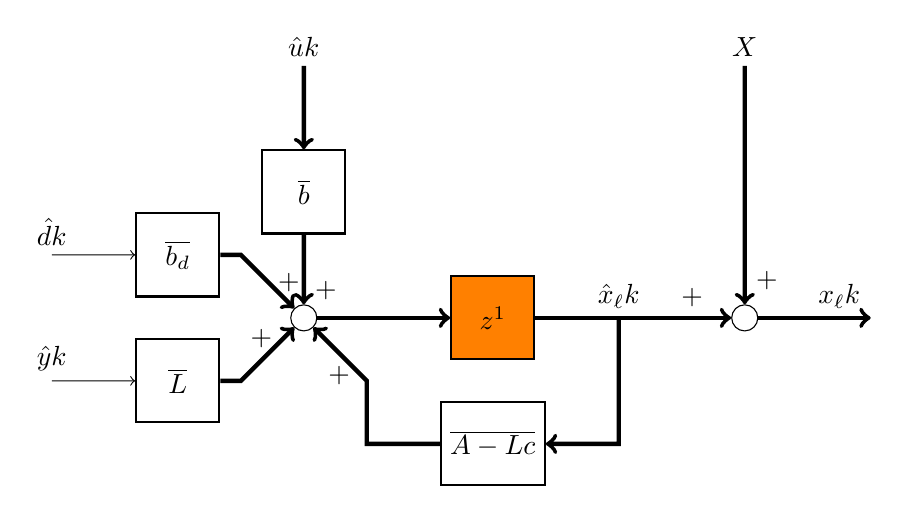
\begin{tikzpicture}[scale = 0.8]
%observer blocks
\draw
	(4,2) node [block] (bb) {$\overline{\boldsymbol{b}}$}
	(4,0) node [sum] (s1) {\suma}
	(7,0) node [block, fill = orange] (i1) {$z^{\minus 1}$}
	(7,-2) node [block] (bA) {$\overline{\squarey{\boldsymbol{A} - \boldsymbol{L}\boldsymbol{c}}}$}
	(2,-1) node [block] (bL) {$\overline{\boldsymbol{L}}$}
	(2,1) node [block] (bbD) {$\overline{\boldsymbol{b}_d}$}
	(11,0) node [sum] (s2) {\suma};
%observer lines
\draw[->, ultra thick] (4,4) -- (bb);
\draw[->, ultra thick] (bb) -- node [anchor = west, pos = 0.8] {$+$} (s1);
\draw[->, ultra thick] (s1) -- (i1);
\draw[->, ultra thick] (i1) -- node [anchor = south, pos = 0.8] {$+$} (s2);
\draw[->, ultra thick] (9,0) -- (9,-2) -- (bA);
\draw[->, ultra thick] (bA) -- (5,-2) -- (5,-1) -- node [anchor = east, pos = 0.1] {$+$} (s1);
\draw[->, ultra thick] (bbD) -- (3,1) -- node [anchor = south, pos = 0.9] {$+$} (s1);
%more observer lines
\draw[->, ultra thick] (bL) -- (3,-1) -- node [anchor = east, pos = 0.8] {$+$} (s1);
\draw[->] (0,1) -- (bbD);
\draw[->] (0,-1) -- (bL);
\draw[->, ultra thick] (11,4) -- node [anchor = west, pos = 0.9] {$+$} (s2);
\draw[->, ultra thick] (s2) -- (13,0);
%signal labels
\coordinate[label = above:$\hat{d}\squarey{k}$] (d) at (0,1);
\coordinate[label = above:$\hat{\boldsymbol{u}}\squarey{k}$] (u) at (4,4);
\coordinate[label = above:$\hat{y}\squarey{k}$] (yhat) at (0,-1);
\coordinate[label = above:$\boldsymbol{X}$] (bigx) at (11,4);
\coordinate[label = above:$\boldsymbol{x}_\ell\squarey{k}$] (smallx) at (12.5,0);
\coordinate[label = above:$\hat{\boldsymbol{x}}_\ell\squarey{k}$] (hatx) at (9,0);
\end{tikzpicture}
}
\caption{Block diagram of observer discretised under zero-order hold; compare with continuous-time version of Figure~\ref{block:observer2}}
\label{block:observer_discrete}
\end{figure}
%%%%%%%%%%%%%%%%%%%%%%%%%%%%%%%%%%%%%%%%%%%%%%%%%%%%%%%%%%%%%%%%%%%%%%%%%%%%%%%%
\subsubsection{Discretising integral action - forward-euler integration}
Discrete time integral action under the forward-euler method is achieved through the transfer function
\begin{align}\label{eqn:integral_discrete}
H(z) = \frac{T_s}{z - 1}.
\end{align}
In terms of block diagrams, the integral action integrator block $1/s$ is replaced with $H(z) = \frac{T_s}{z - 1}$, assuming the control inputs are constant over the sampling period $T_s$.
%%%%%%%%%%%%%%%%%%%%%%%%%%%%%%%%%%%%%%%%%%%%%%%%%%%%%%%%%%%%%%%%%%%%%%%%%%%%%%%%
\subsubsection{Augmented control loop - discrete time}\label{sec:control_ultimate}
The block diagram for the resulting fully-discrete control loop is given in Figure~\ref{block:control_discrete}.
\begin{figure}[H]
\centering
\fbox{
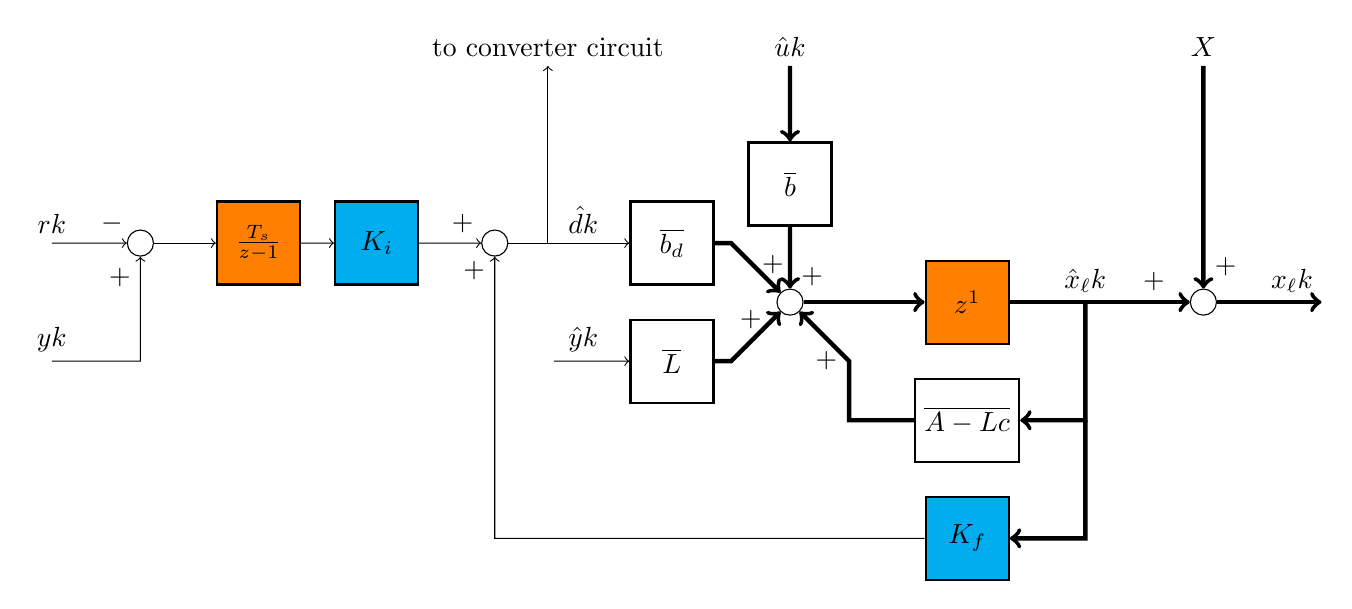
\begin{tikzpicture}[scale = 0.75]
% blocks
\draw
	(4,2) node [block] (bb) {$\overline{\boldsymbol{b}}$}
	(4,0) node [sum] (s1) {\suma}
	(7,0) node [block, fill = orange] (i1) {$z^{\minus 1}$}
	(7,-2) node [block] (bA) {$\overline{\squarey{\boldsymbol{A} - \boldsymbol{L}\boldsymbol{c}}}$}
	(2,-1) node [block] (bL) {$\overline{\boldsymbol{L}}$}
	(2,1) node [block] (bbD) {$\overline{\boldsymbol{b}_d}$}
	(11,0) node [sum] (s2) {\suma}
	(7,-4) node [block, fill = cyan] (bKf) {$\minus \boldsymbol{K}_f$};
% observer lines
\draw[->, ultra thick] (4,4) -- (bb);
\draw[->, ultra thick] (bb) -- node [anchor = west, pos = 0.8] {$+$} (s1);
\draw[->, ultra thick] (s1) -- (i1);
\draw[->, ultra thick] (i1) -- node [anchor = south, pos = 0.8] {$+$} (s2);
\draw[->, ultra thick] (9,0) -- (9,-2) -- (bA);
\draw[->, ultra thick] (bA) -- (5,-2) -- (5,-1) -- node [anchor = east, pos = 0.01] {$+$} (s1);
\draw[->, ultra thick] (bbD) -- (3,1) -- node [anchor = south, pos = 0.85] {$+$} (s1);
% more observer lines
\draw[->, ultra thick] (bL) -- (3,-1) -- node [anchor = east, pos = 0.85] {$+$} (s1);
\draw[->] (0,-1) -- (bL);
\draw[->, ultra thick] (11,4) -- node [anchor = west, pos = 0.9] {$+$} (s2);
\draw[->, ultra thick] (s2) -- (13,0);
% signal labels
\coordinate[label = above:$\hat{d}\squarey{k}$] (d) at (0.5,1);
\coordinate[label = above:$\hat{\boldsymbol{u}}\squarey{k}$] (u) at (4,4);
\coordinate[label = above:$\hat{y}\squarey{k}$] (yhat) at (0.5,-1);
\coordinate[label = above:$\boldsymbol{X}$] (bigx) at (11,4);
\coordinate[label = above:$\boldsymbol{x}_\ell\squarey{k}$] (smallx) at (12.5,0);
\coordinate[label = above:$\hat{\boldsymbol{x}}_\ell\squarey{k}$] (hatx) at (9,0);
\coordinate[label = above:$r\squarey{k}$] (r) at (-8.5,1);
\coordinate[label = above:$y\squarey{k}$] (r) at (-8.5,-1);
% integrator blocks
\draw
    (-1,1) node [sum] (s5) {\suma}
	(-3,1) node [block, fill = cyan] (bKi) {$\minus K_i$}
	(-5,1) node [block, fill = orange] (i2) {$\frac{T_s}{z - 1}$}
	(-7,1) node [sum] (s4) {\suma};
% feedback lines
\draw[->, ultra thick] (9,-2) -- (9,-4) -- (bKf);
\draw[->] (bKf) -- (-1,-4) -- node [anchor = east, pos = 0.95] {$+$} (s5);
\draw[->] (s5) -- (bbD);
% integrator lines
\draw[->] (-8.5,1) -- node [anchor = south, pos = 0.8] {$-$} (s4);
\draw[->] (s4) -- (i2);
\draw[->] (i2) -- (bKi);
\draw[->] (bKi) -- node [anchor = south, pos = 0.7] {$+$} (s5);
\draw[->] (-8.5,-1) -- (-7,-1) -- node [anchor = east, pos = 0.8] {$+$} (s4);
% more lines
\draw[->] (-0.1,1) -- (-0.1,4);
% more labels
\coordinate[label = above:{to converter circuit}] (dout) at (-0.1,4);
\end{tikzpicture}
}
\caption[Caption without FN]{Block diagram of achieving discrete-time observer state feedback and integral action acting on the model of Equation~(\ref{eqn:timevarying2}); compare with continuous-time version of Figure~\ref{block:integral}\footnotemark}
\label{block:control_discrete}
\end{figure}
\footnotetext{Don't forget the note on page~\pageref{block:feedback} regarding the meaning of `to converter circuit'.}
%%%%%%%%%%%%%%%%%%%%%%%%%%%%%%%%%%%%%%%%%%%%%%%%%%%%%%%%%%%%%%%%%%%%%%%%%%%%%%%%
\subsection{Control summary}
At integer time step $k$:
\begin{itemize}
\item $r\squarey{k}$: input reference signal/desired output voltage
\item $y\squarey{k}$: output voltage as measured by ADC
\item $\hat{d}\squarey{k}$: duty ratio perturbation to be sent to update PWM signal
\item $\hat{y}\squarey{k}$: output voltage perturbation from steady-state calculated according to
    \begin{itemize}
    \item $\hat{y}\squarey{k} = y\squarey{k} - \, Y$
    \end{itemize}
\item $\hat{\boldsymbol{u}}\squarey{k}$: input vector perturbation from steady-state calculated according to
    \begin{itemize}
    \item $\hat{\boldsymbol{u}}\squarey{k} = \boldsymbol{u}\squarey{k} - \, \boldsymbol{U}$
    \item note that only the first element of $\hat{\boldsymbol{u}}\squarey{k}$ changes while running the control loop; diode forward voltage drop is considered to be unchanging under forward bias
    \end{itemize}
\item $\hat{\boldsymbol{x}}_\ell\squarey{k}$: estimated state vector perturbation from steady-state
    \begin{itemize}
    \item used for full-state feedback control
    \end{itemize}
\item $\boldsymbol{x}_\ell\squarey{k}$: estimated state vector
    \begin{itemize}
    \item vector containing estimates of state variables
    \end{itemize}
\end{itemize}
%%%%%%%%%%%%%%%%%%%%%%%%%%%%%%%%%%%%%%%%%%%%%%%%%%%%%%%%%%%%%%%%%%%%%%%%%%%%%%%%
\subsection{Notes on realising the control loop in hardware}\label{sec:hardware_for_control}
The basic modules required for hardware implementation of our control loop will be introduced presently.
\paragraph{Measuring $v_g(t)$ and $y(t)$: op-amp sensing circuitry}
\paragraph{Writing the control signal to the DC-DC converter: achieving PWM functionality in hardware}
\paragraph{Iterating the control loop: using a microcontroller to process measurements and to calculate the control signals}
%%%%%%%%%%%%%%%%%%%%%%%%%%%%%%%%%%%%%%%%%%%%%%%%%%%%%%%%%%%%%%%%%%%%%%%%%%%%%%%%
%%%%%%%%%%%%%%%%%%%%%%%%%%%%%%%%%%%%%%%%%%%%%%%%%%%%%%%%%%%%%%%%%%%%%%%%%%%%%%%%